% \documentclass[border=1mm, class=article preview]{standalone}
\documentclass[border=5pt,tikz]{standalone}
\usepackage{tikz}
\usetikzlibrary{calc,patterns,decorations.pathmorphing,decorations.markings}

\begin{document}

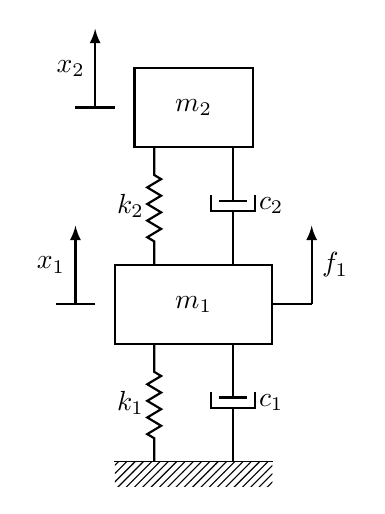
\begin{tikzpicture}
% TikZ Styles
\tikzstyle{mass}=[draw,outer sep=0pt,thick]
\tikzstyle{spring}=[thick,decorate,decoration={zigzag,pre length=0.3cm,post length=0.3cm,segment length=6}]
\tikzstyle{damper}=[thick,decoration={markings,  
  mark connection node=dmp,
  mark=at position 0.5 with 
  {
    \node (dmp) [thick,inner sep=0pt,transform shape,rotate=-90,minimum width=15pt,minimum height=3pt,draw=none] {};
    \draw [thick] ($(dmp.north east)+(2pt,0)$) -- (dmp.south east) -- (dmp.south west) -- ($(dmp.north west)+(2pt,0)$);
    \draw [thick] ($(dmp.north)+(0,-5pt)$) -- ($(dmp.north)+(0,5pt)$);
  }
}, decorate]
\tikzstyle{ground}=[fill,pattern=north east lines,draw=none,minimum width=0.75cm,minimum height=0.3cm]
% Actual Drawing
\node (m2) [mass,minimum width=1.5cm,minimum height=1cm] {$m_2$};
\node (m1) at (m2.south) [mass,yshift=-1.5cm,anchor=north,minimum width=2cm,minimum height=1cm] {$m_1$};
\node (ground) at (m1.south) [ground,yshift=-1.5cm,anchor=north,minimum width=2cm] {};
\draw (ground.north west) -- (ground.north east);
\draw [spring] ([xshift=-0.5cm] ground.north) -- ([xshift=-0.5cm] $(m1.south east)!(ground.north)!(m1.south west)$) node[midway, left]{$k_1$};
\draw [damper] ([xshift=0.5cm] ground.north) -- ([xshift=0.5cm] $(m1.south east)!(ground.north)!(m1.south west)$) node[midway, right,xshift=2mm]{$c_1$};
\draw [spring] (m1.135) -- ($(m2.south east)!(m1.135)!(m2.south west)$) node[midway, left]{$k_2$};
\draw [damper] (m1.45) -- ($(m2.south east)!(m1.45)!(m2.south west)$) node[midway, right,xshift=2mm]{$c_2$};
\draw [thick] (m1.east) -- +(0.5cm,0);
\draw [-latex,thick] ([xshift=0.5cm]m1.east) -- +(0,1cm) node[midway, right]{$f_1$};
\draw [thick] ([xshift=-0.25cm]m1.west) -- +(-0.5cm,0);
\draw [-latex,thick] ([xshift=-0.5cm]m1.west) -- +(0,1cm) node[midway, left]{$x_1$};
\draw [thick] ([xshift=-0.25cm]m2.west) -- +(-0.5cm,0);
\draw [-latex,thick] ([xshift=-0.5cm]m2.west) -- +(0,1cm) node[midway, left]{$x_2$};
\end{tikzpicture}

\end{document}